\section{Implementation details}

Both algorithms described in this paper were implemented using C++20 for an open-source KOALA NetworKit library \cite{koala-networkit}.
\subsection{KOALA NetworKit}
According to library README file the KOALA NetworKit is a hybrid library that combines the efficiency and scalability of the NetworKit platform with the rich set of classical graph algorithms provided by the KOALA library. NetworKit is a modern, open-source C++ library focused on fast analysis and mining of large-scale networks, offering high-performance implementations of algorithms for centrality, community detection, graph metrics, and random graph generation, with extensive use of parallelization and efficient data structures. KOALA, developed at Gdansk University of Technology, supplements this toolkit with a comprehensive collection of algorithms for classical discrete optimization and graph theory problems, including advanced procedures for coloring, flows, scheduling, and graph recognition. KOALA NetworKit thus provides a unified interface for both large-scale graph analytics and specialized combinatorial algorithms, making it a versatile tool for both theoretical and practical graph research.

The contribution of this work to the Open Source KOALA NetworKit library is mainly in three file:
\begin{itemize}
    \item \texttt{cpp/planar\_sssp/SuitableRDivision.cpp} - implementation of \Cref{findSuitable} and implementation of planar separator algorithm,
    
    \item \texttt{cpp/planar\_sssp/FredericksonPlanarSSSP.cpp} - implementation of \Cref{FredericksonSSSP} (class \texttt{FredericksonPlanarSSSP}),
    
    \item \texttt{cpp/planar\_sssp/HenzingerPlanarSSSP.cpp} - implementation of \Cref{henzingerFormal} (class \texttt{HenzingerPlanarSSSP}).
\end{itemize}

\subsection{Suitable r-division}
One important implementation detail has been omitted throughout this work and in \cite{frederickson}, namely, how to efficiently merge regions.

The division is implemented as a vector of vectors. While this representation is convenient to use, it presents a challenge for greedy merging of regions. Initially, regions can be of size $O(1)$, which means that a single region may be merged many times with others before reaching the desired size. To ensure a linear time bound, it is sufficient to always merge the smaller region into the larger one. In this approach, whenever two regions are merged, the nodes from the smaller region are moved into the larger one. Although a single node may be moved between regions multiple times, by always merging the smaller region into the larger, the total number of moves over all nodes is amortized and remains $O(n)$.

For the planar separator implementation, the Fundamental Cycle Separator was used. This choice is motivated by its simplicity of implementation and its favorable experimental separator sizes.

\subsection{Henzinger's SSSP}
There is a major optimization that can be applied to improve the efficiency of \Cref{henzingerFormal}, we can eliminate almost all recursive calls. Below, we present an iterative and simplified version of \Cref{henzingerFormal}, based on the brief description in \cite{henzinger}. The iterative approach is particularly well-suited to the three-level version of the algorithm described in the paper. In the recursive variant, certain calls to the \textsc{Process} procedure serve primarily a theoretical purpose, especially for level 2 regions. Additionally, the priority queues corresponding to single atomic regions have been omitted.

\begin{algorithm}[H]
\caption{\textsc{OptimizedSimplifiedHenzingerSSSP}}\label{henzingersimplified}
\begin{algorithmic}[1]
\Require Planar graph $G=(V,E)$, source node $s$
\Ensure Shortest path distances $d(v)$ from $s$ to all $v \in V$

\While{$\textsc{minKey}(Q) < \infty$}
    \State $R \gets \textsc{minItem}(Q)$
    \For{$i = 1$ to $\log n$}
        \State $u v \gets \textsc{minItem}(Q(R))$
        \State $d[v] \gets d[u] + \text{w}(u v)$
        \State $\textsc{update}(Q(R), (u,v), \infty)$
        \ForAll{outgoing edge $(v,w)$ of $v$ in $R$}
            \ForAll{$R'$ that contain edge $v w$}
            \State $\textsc{update}(Q(R'), (v,w), d[v])$
            \If{\textsc{minKey}(Q(R')) changed}
            \State $\textsc{update}(Q, R', \textsc{minKey}(Q(R')))$
            \EndIf
            \EndFor
        \EndFor
    \EndFor
    \State $\textsc{update}(Q, R, \textsc{minKey}(Q(R)))$
\EndWhile
\State \Return{$d[v]$ for all $v \in V$}
\end{algorithmic}
\end{algorithm}

One more optimization that can be done as mentioned in \cite{henzinger} is to use priority queue that allows for deletion and insertion of regions. Because simplified version of the algorithm uses only three levels of division, finding the appropriate queue is not problematic and results in improvement of a constant. Unfortunately this optimization does not result in improved complexity.

For the implementation of priority queue standard \texttt{std::set} has been used with extra caching of the smallest key to ensure constant lookup times.

\section{Benchmarks}
Running time of both algorithms have been tested with following experiments:
\begin{enumerate}
\item grid, triangular grid, hexagonal grid, and single path graphs with fewer than $10 000$ nodes were tested with randomly generated edge weights using the suitable $r$-division algorithm (see \Cref{fig:grid,fig:hex,fig:line,fig:trig}),
\item a hexagonal grid with more than 1,000,000 nodes was tested using a precalculated division (see \Cref{fig:PrecalculatedHenzinger}),
\item the effect of different division parameters was examined for grid, hexagonal grid, and triangular grid graphs (see \Cref{fig:Pgrid,fig:Phex,fig:Ptrig}),
\item subgraphs with fewer than 10,000 nodes were sampled from the New York City map dataset \cite{ny} (see \Cref{fig:city}),
\item maximal planar graphs(see \Cref{fig:max}).
\end{enumerate}

All edge weights were generated randomly by sampling from a uniform distribution over the range $[0, 1000]$. The subgraphs of the NY city map were created by randomly selecting nodes and then running BFS until the desired size was reached. Maximal planar graphs were generated by first creating a cycle of the desired number of vertices and then triangulating the graph by adding edges as long as possible without breaking graphs planarity.

\section{Results}

\begin{figure}[H]
    \centering
    \begin{adjustbox}{center}
        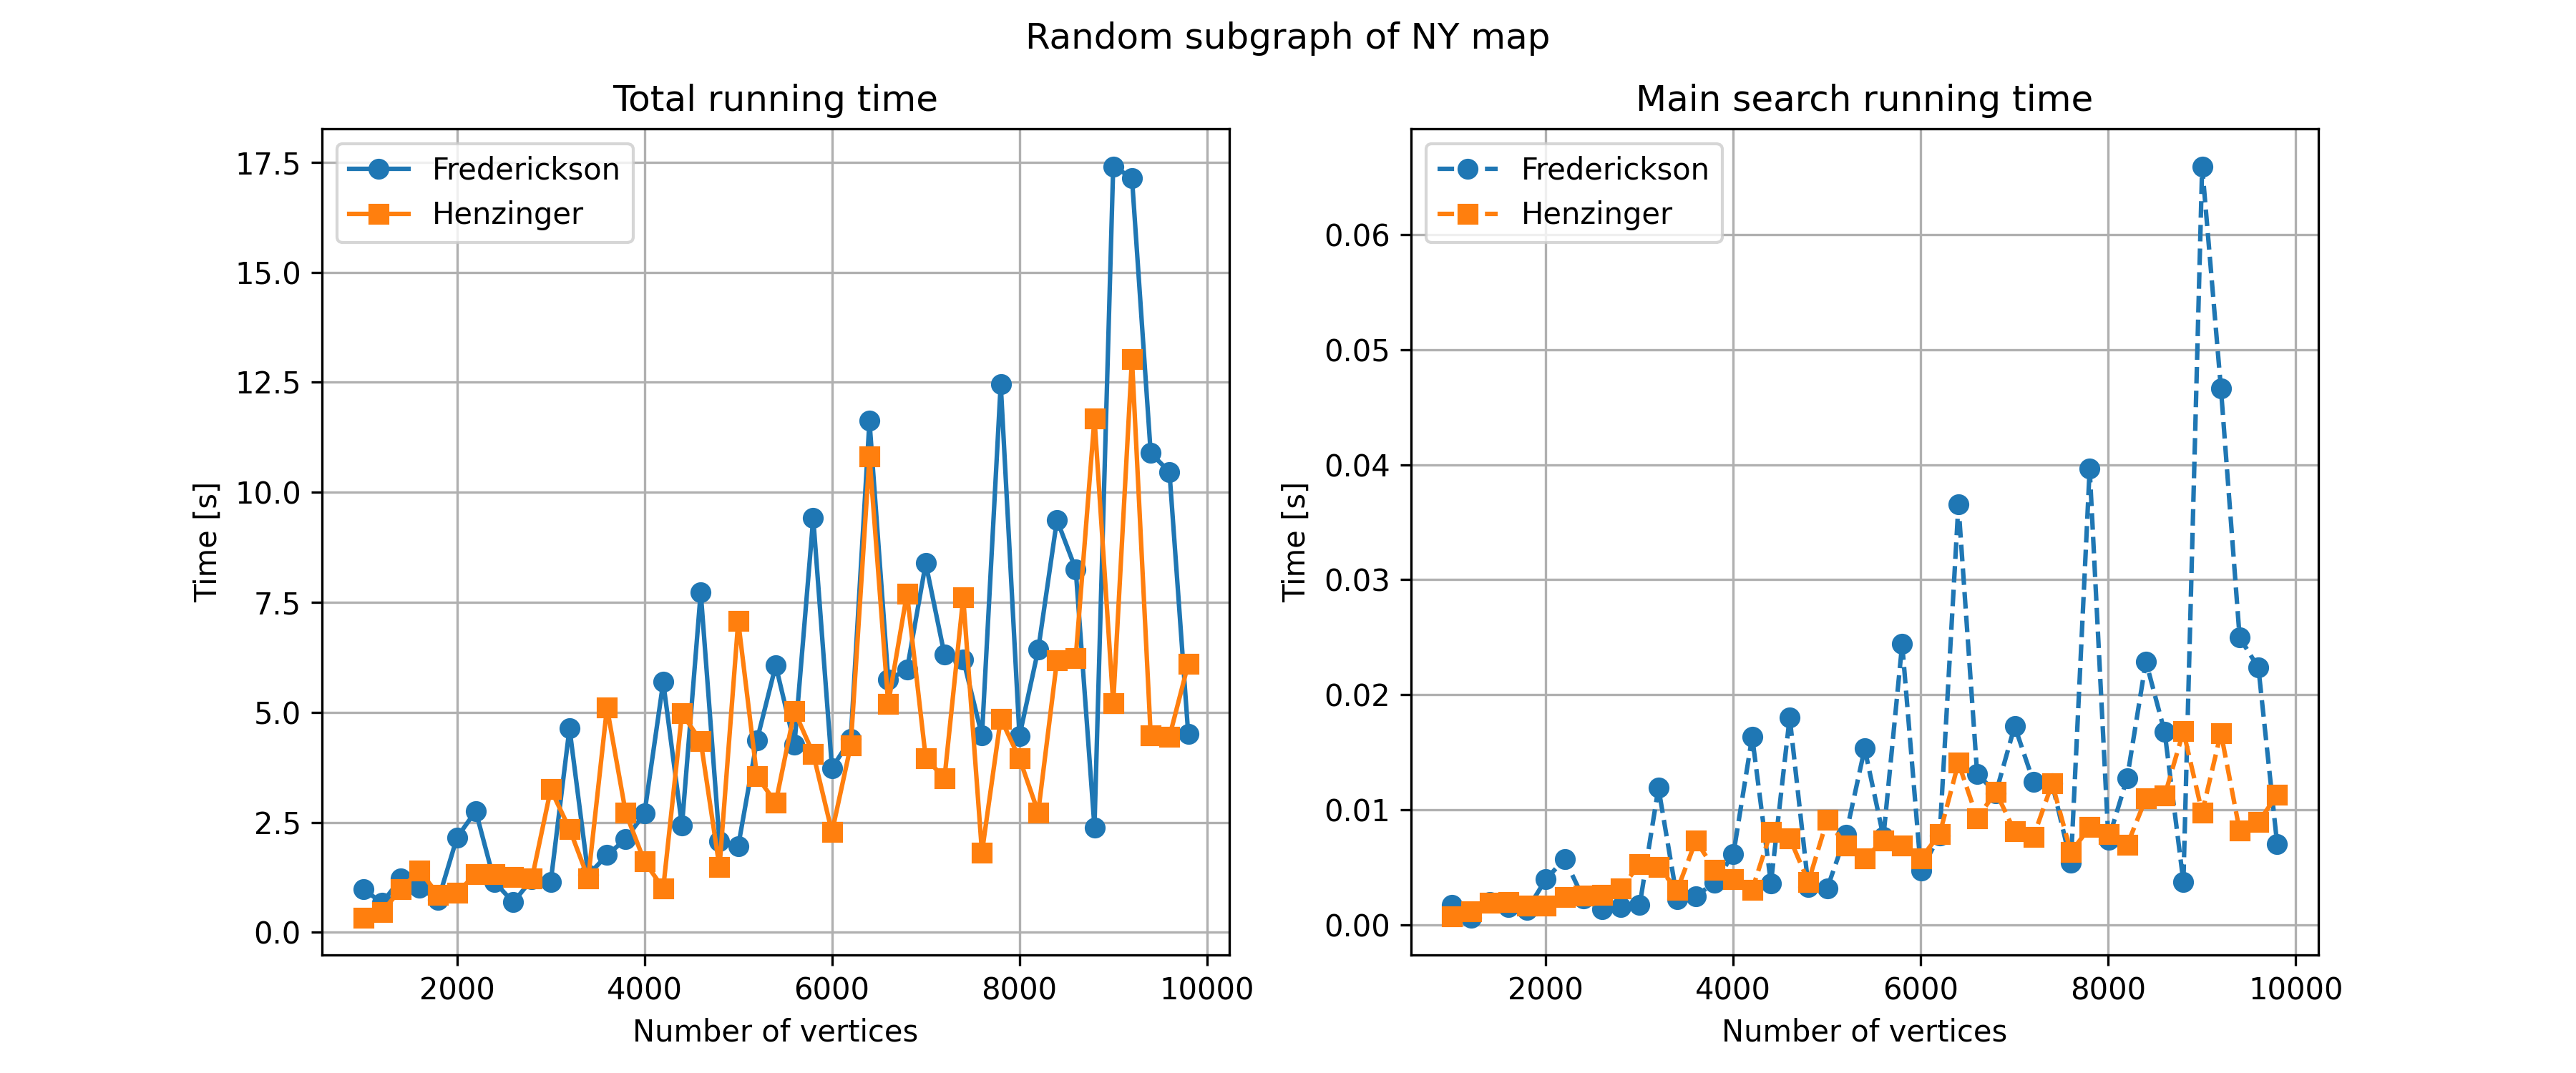
\includegraphics[width=1.4\textwidth]{charts/city.png}
    \end{adjustbox}
    \caption{}
    \label{fig:city}
\end{figure}

\begin{figure}[H]
    \centering
    \begin{adjustbox}{center}
        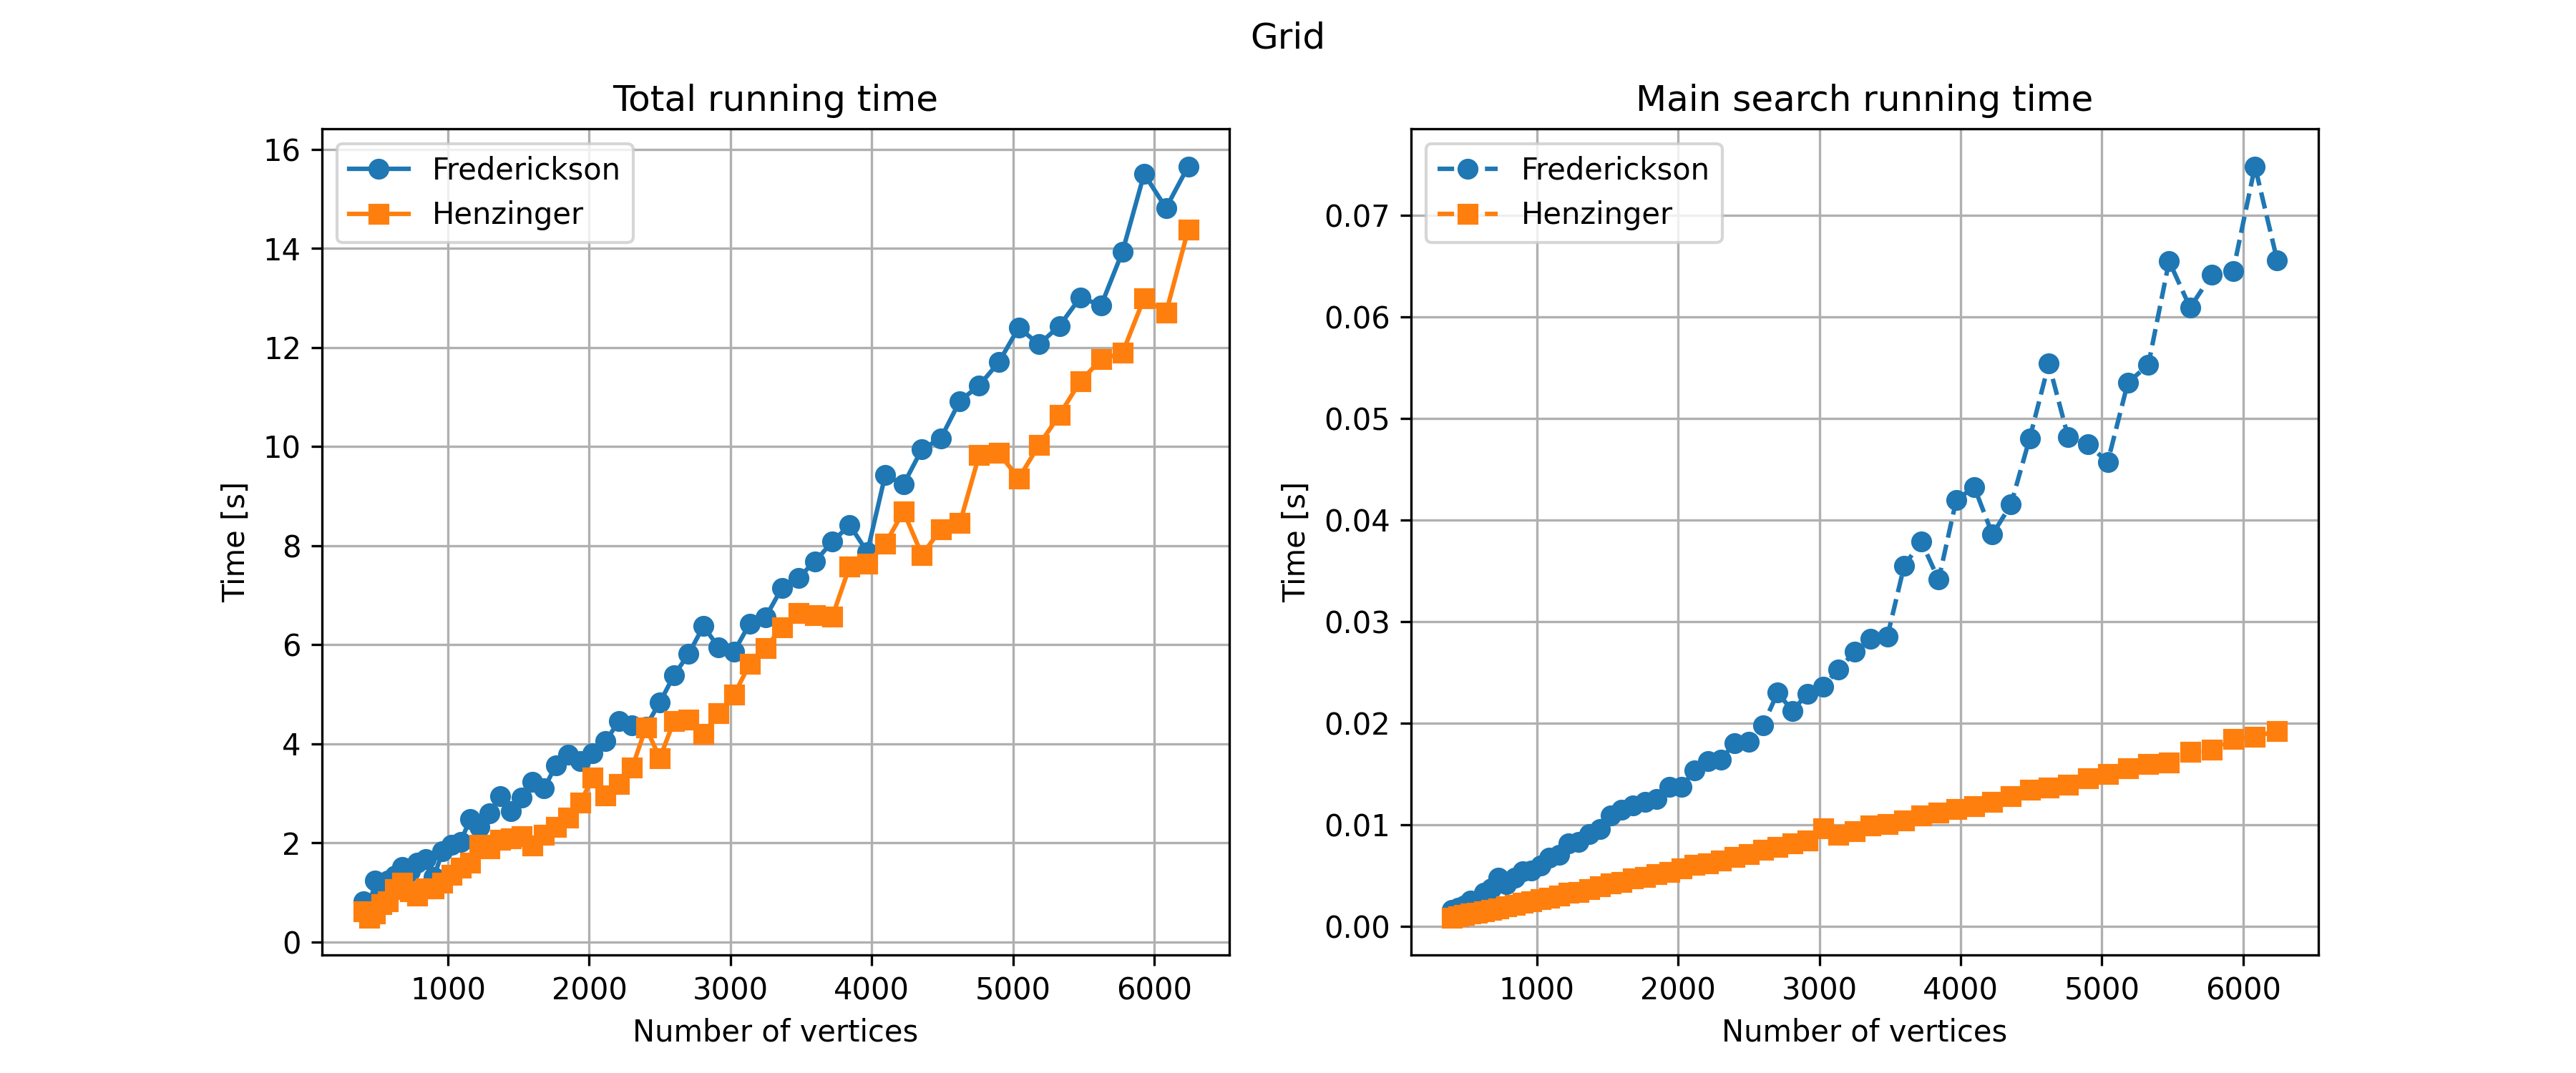
\includegraphics[width=1.4\textwidth]{charts/grid.png}
    \end{adjustbox}
    \caption{}
    \label{fig:grid}
\end{figure}

\begin{figure}[H]
    \centering
    \begin{adjustbox}{center}
        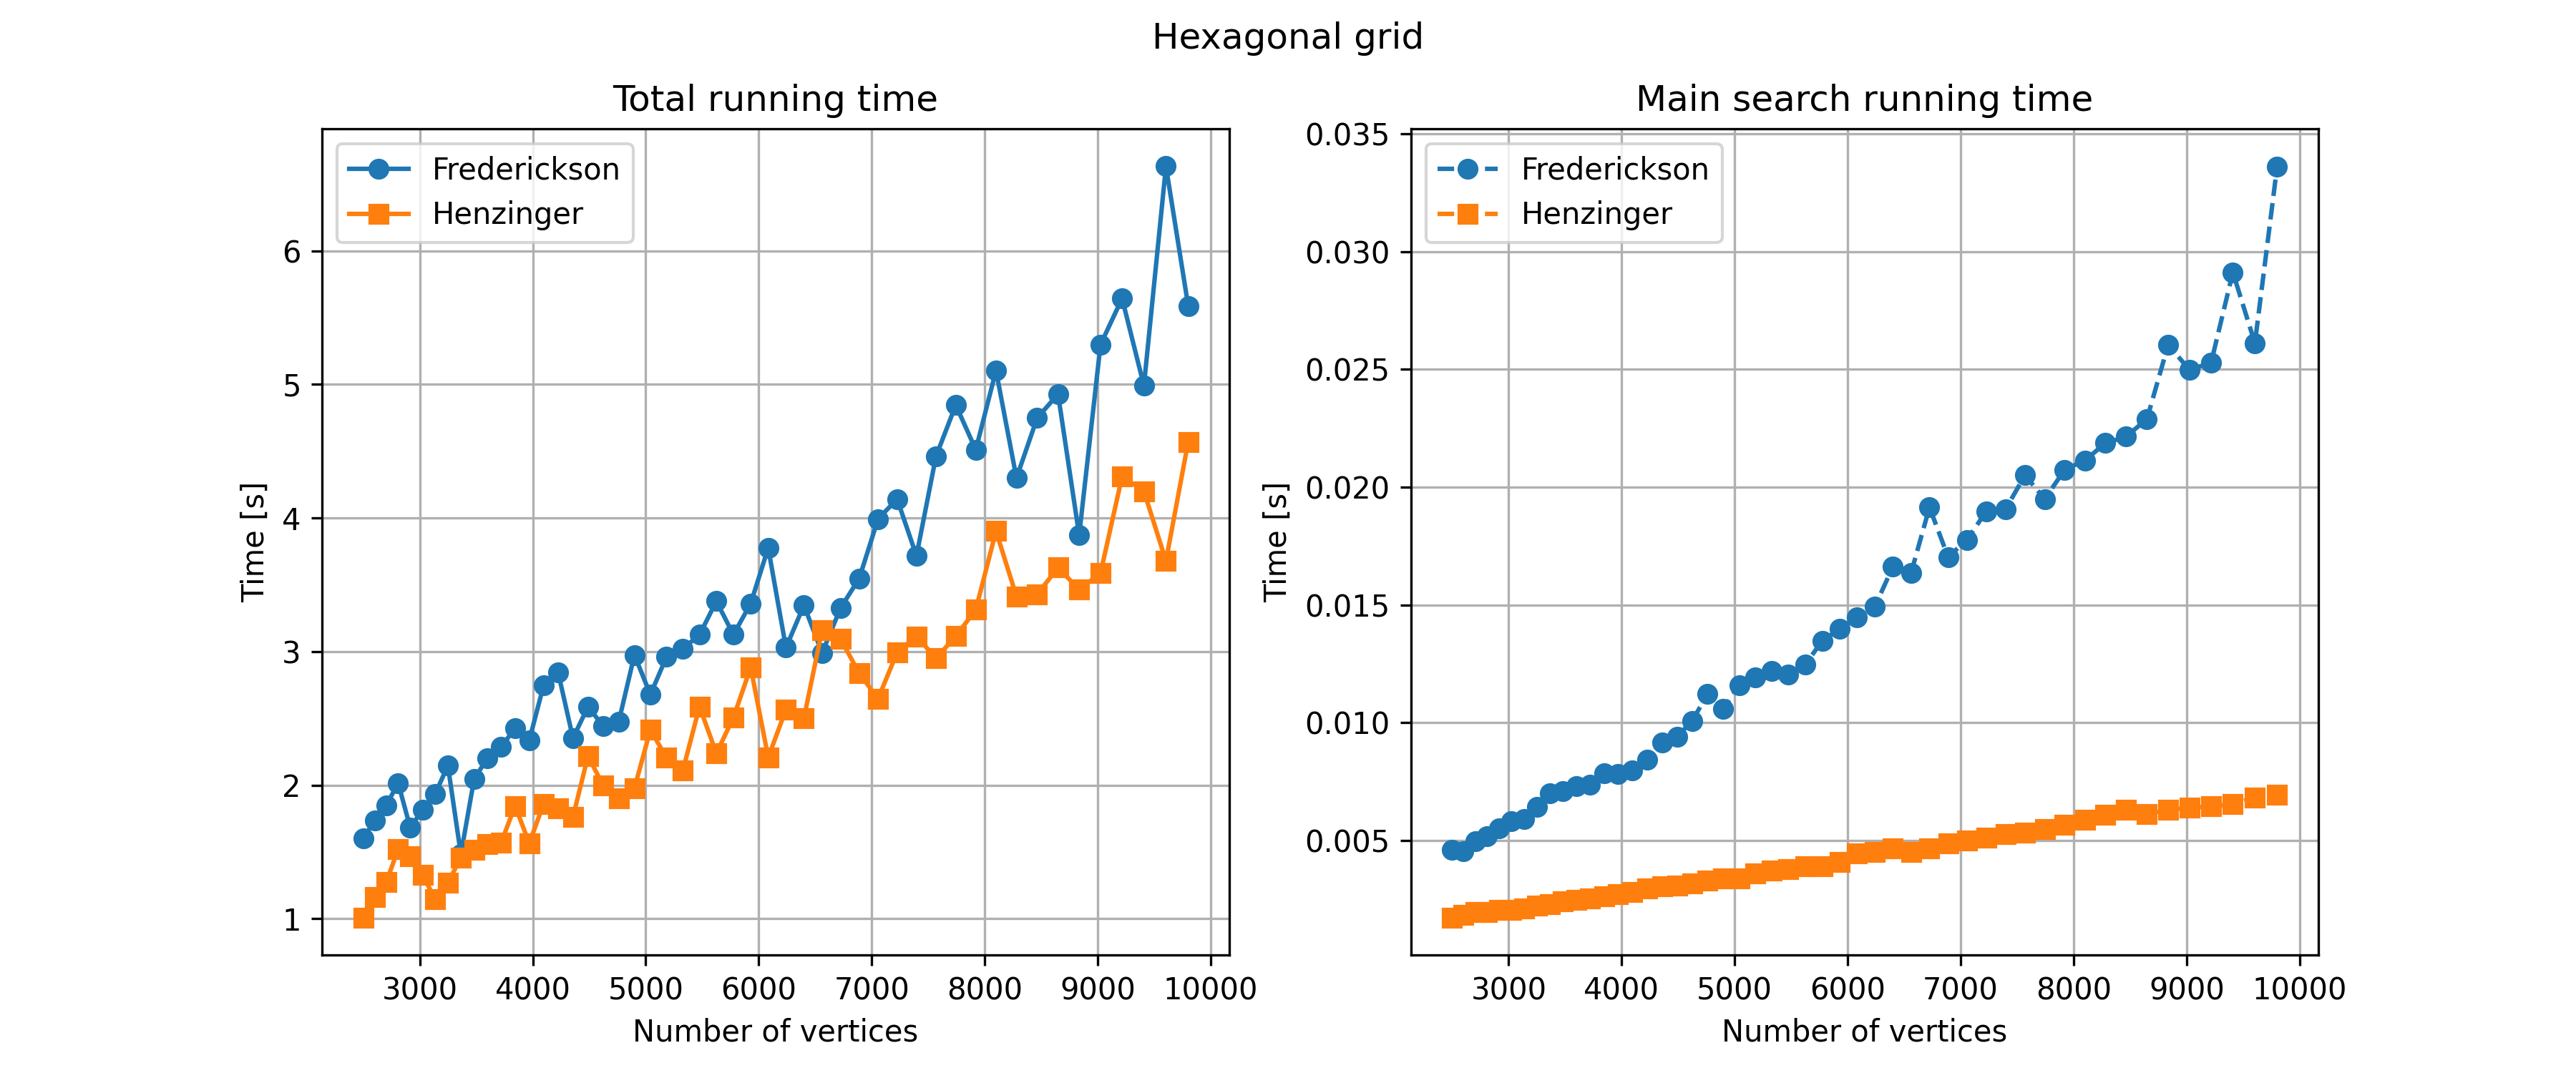
\includegraphics[width=1.4\textwidth]{charts/hex.png}
    \end{adjustbox}
    \caption{}
    \label{fig:hex}
\end{figure}

\begin{figure}[H]
    \centering
    \begin{adjustbox}{center}
        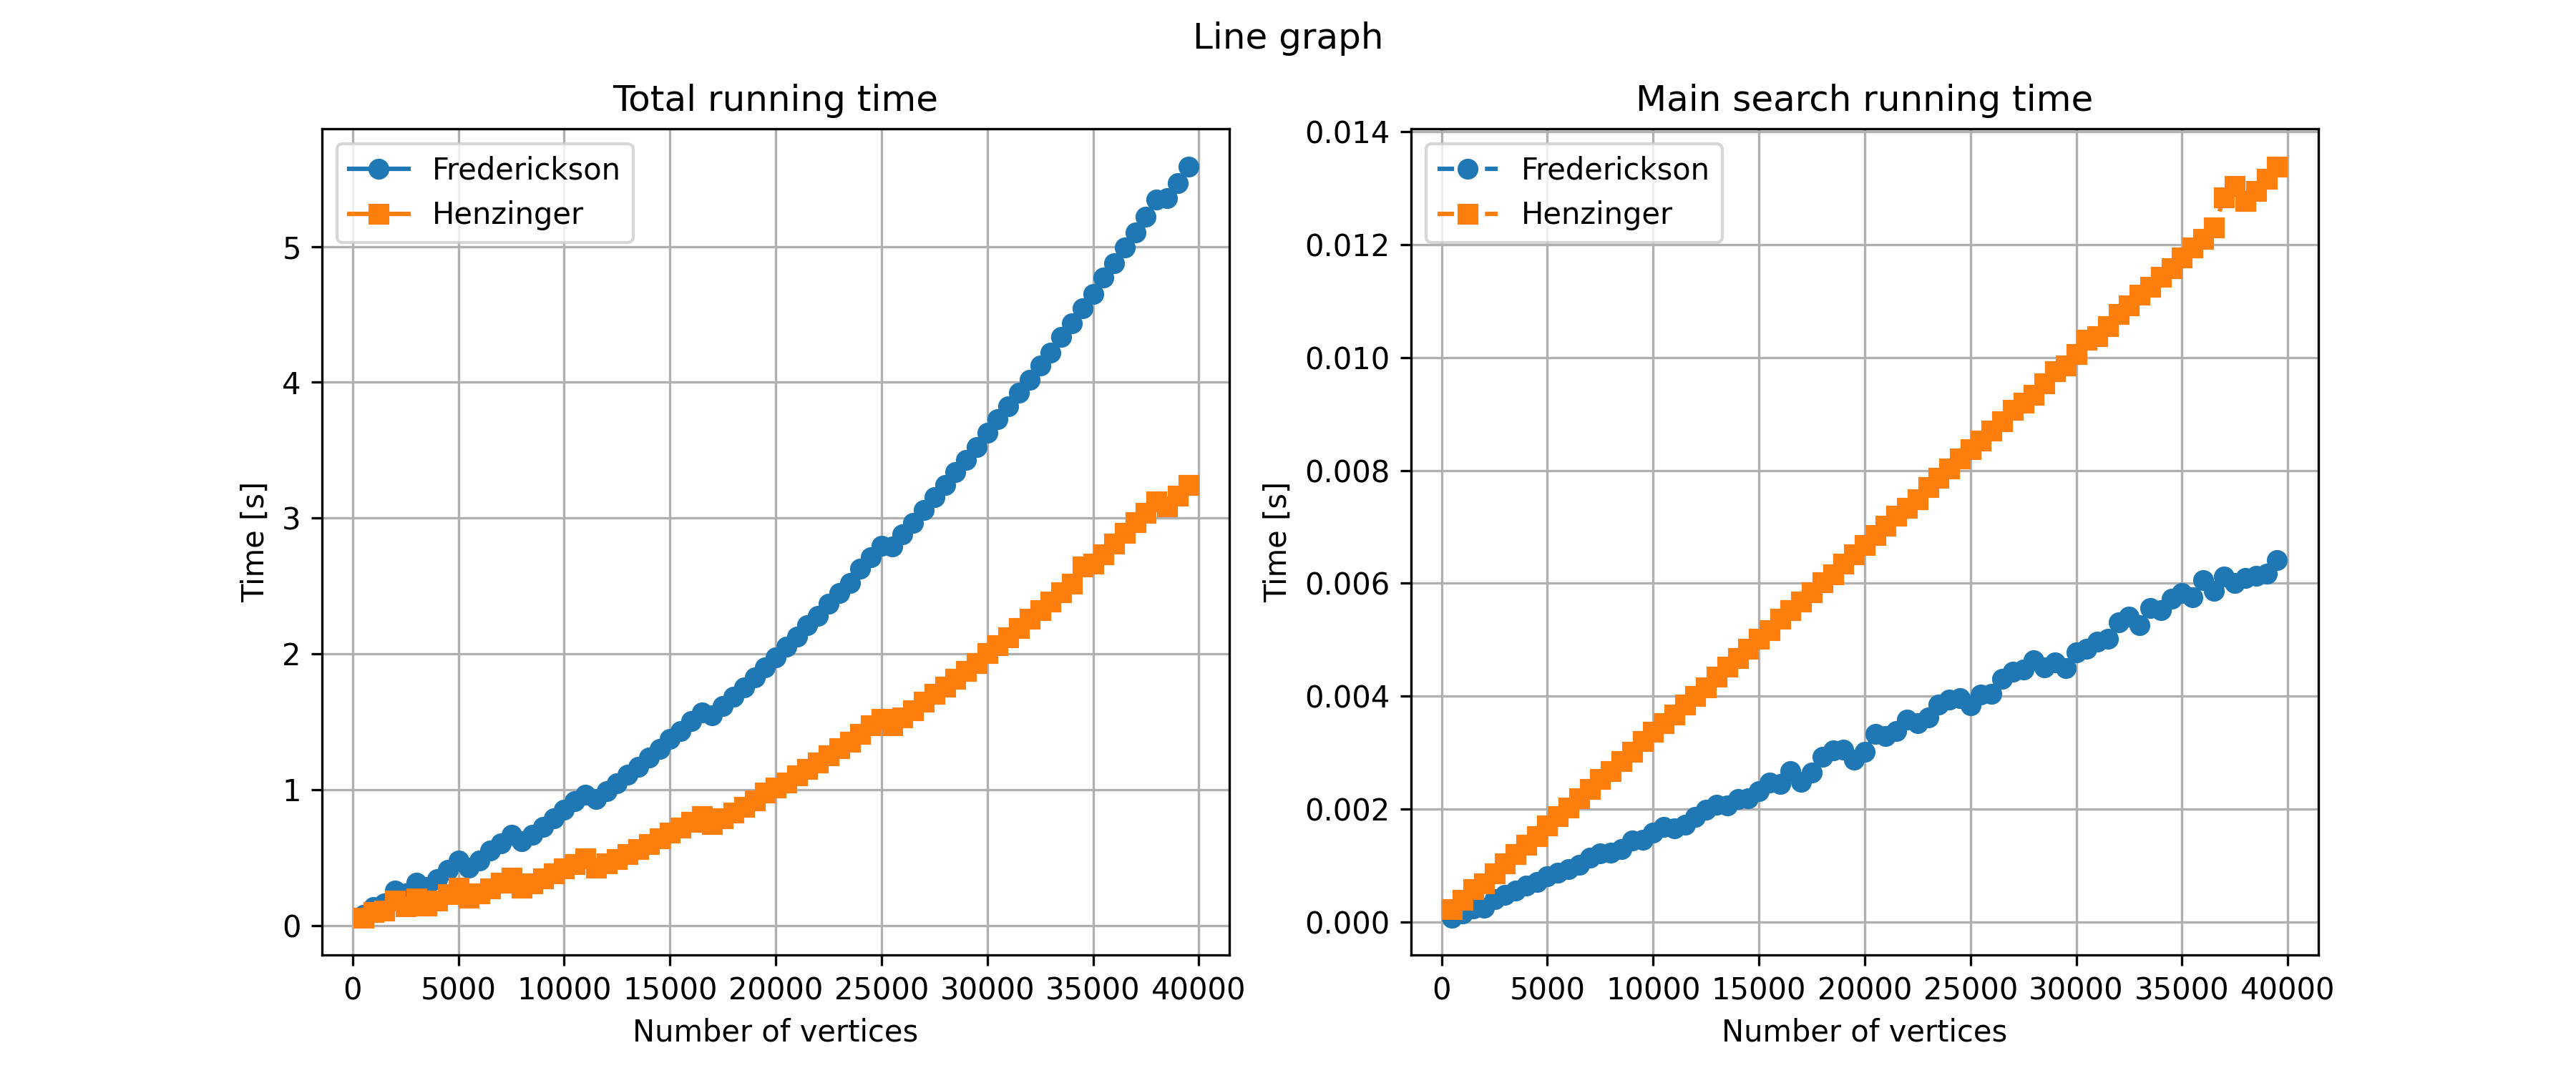
\includegraphics[width=1.4\textwidth]{charts/line.png}
    \end{adjustbox}
    \caption{}
    \label{fig:line}
\end{figure}

\begin{figure}[H]
    \centering
    \begin{adjustbox}{center}
        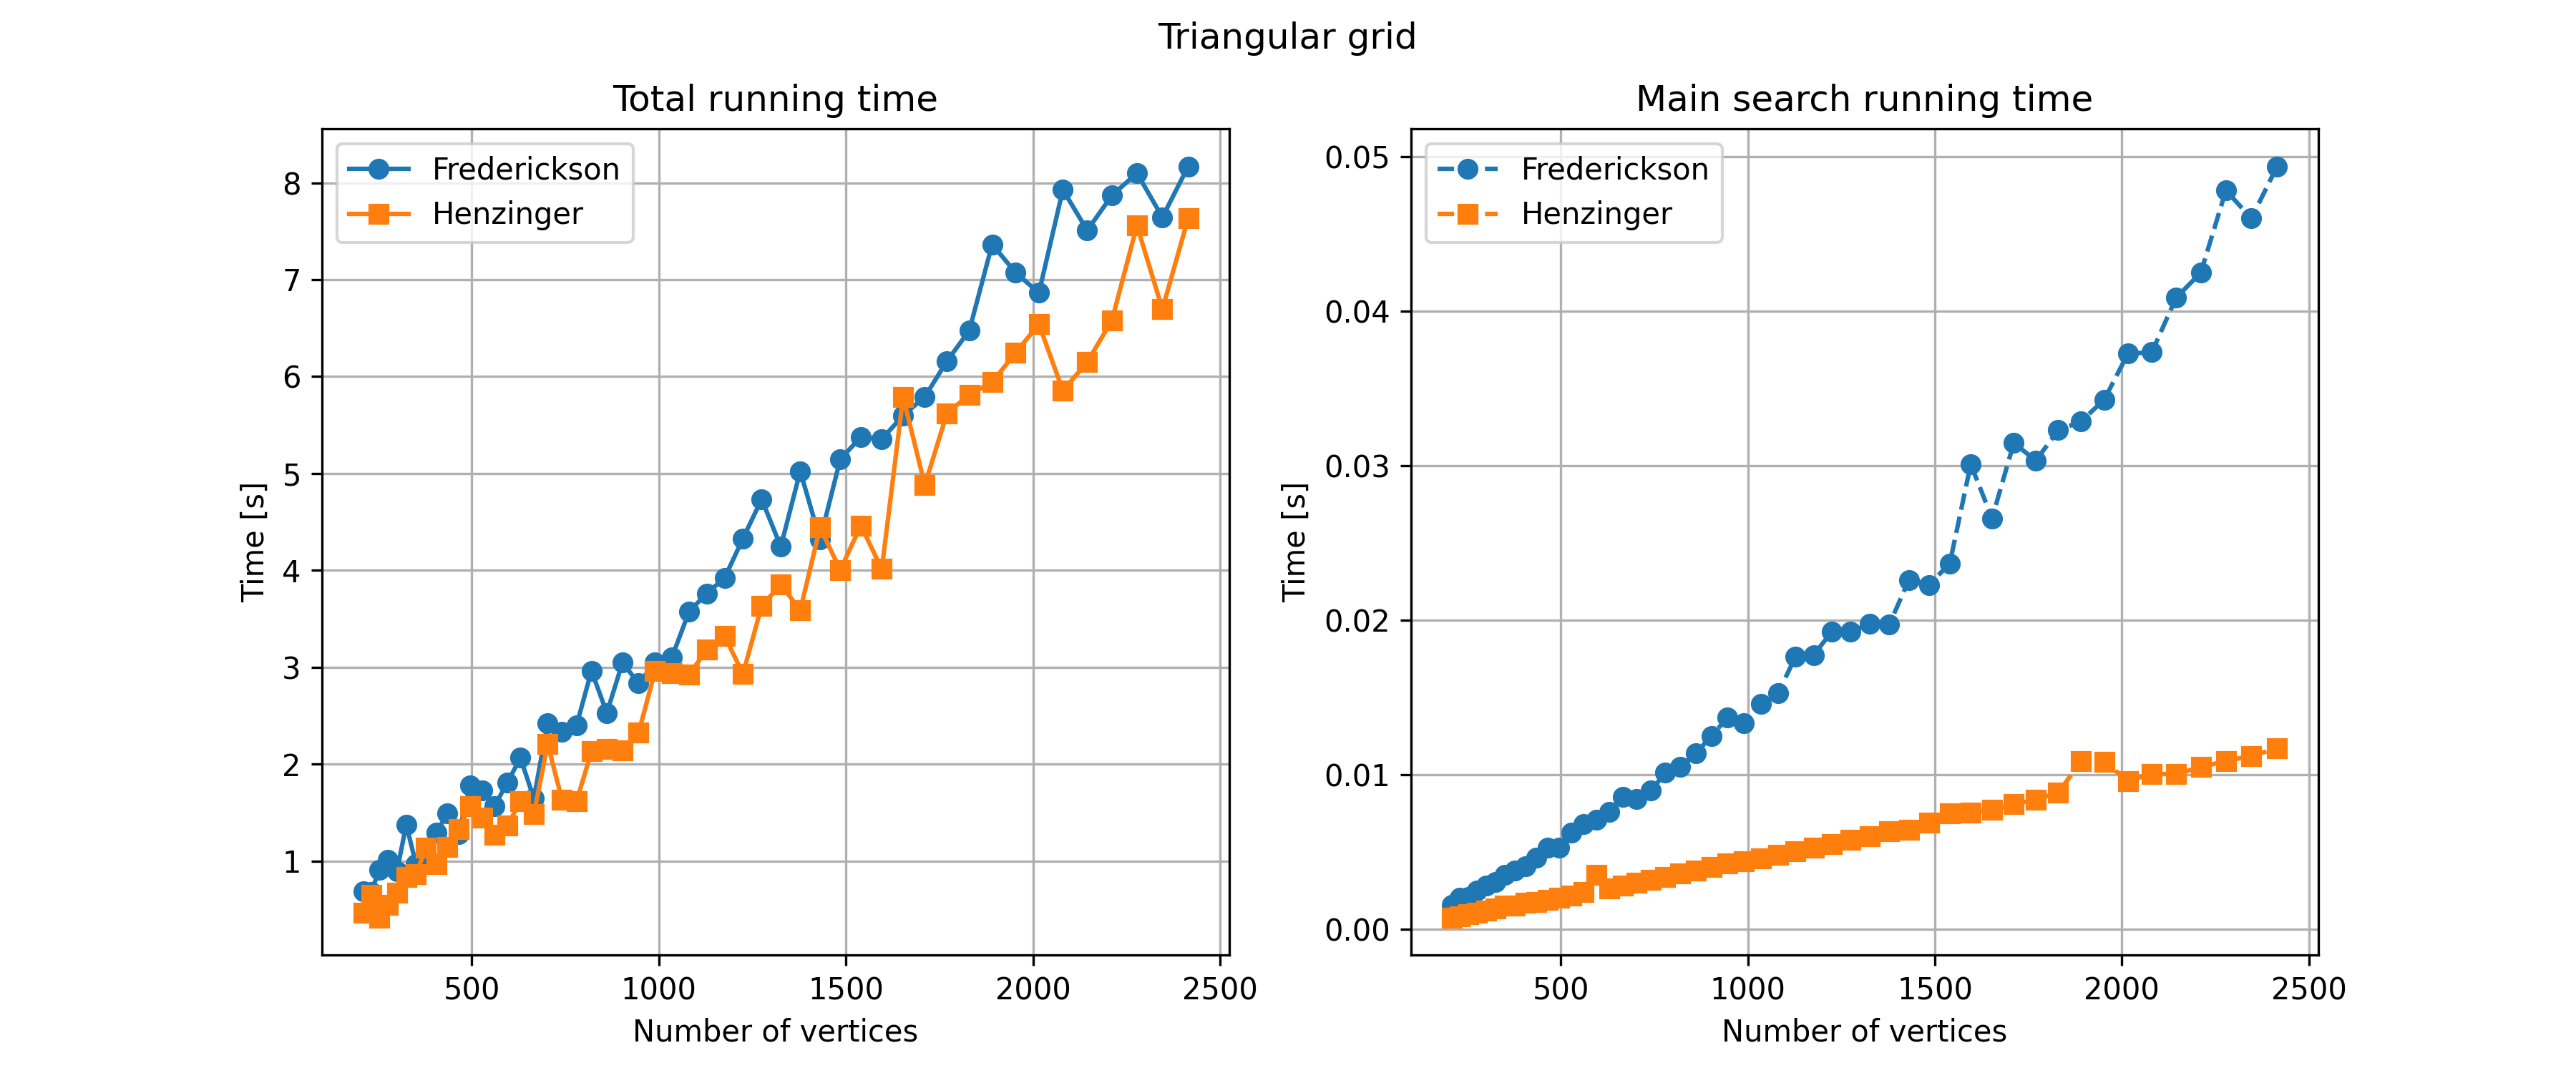
\includegraphics[width=1.4\textwidth]{charts/trig.png}
    \end{adjustbox}
    \caption{}
    \label{fig:trig}
\end{figure}

\begin{figure}[H]
    \centering
    \begin{adjustbox}{center}
        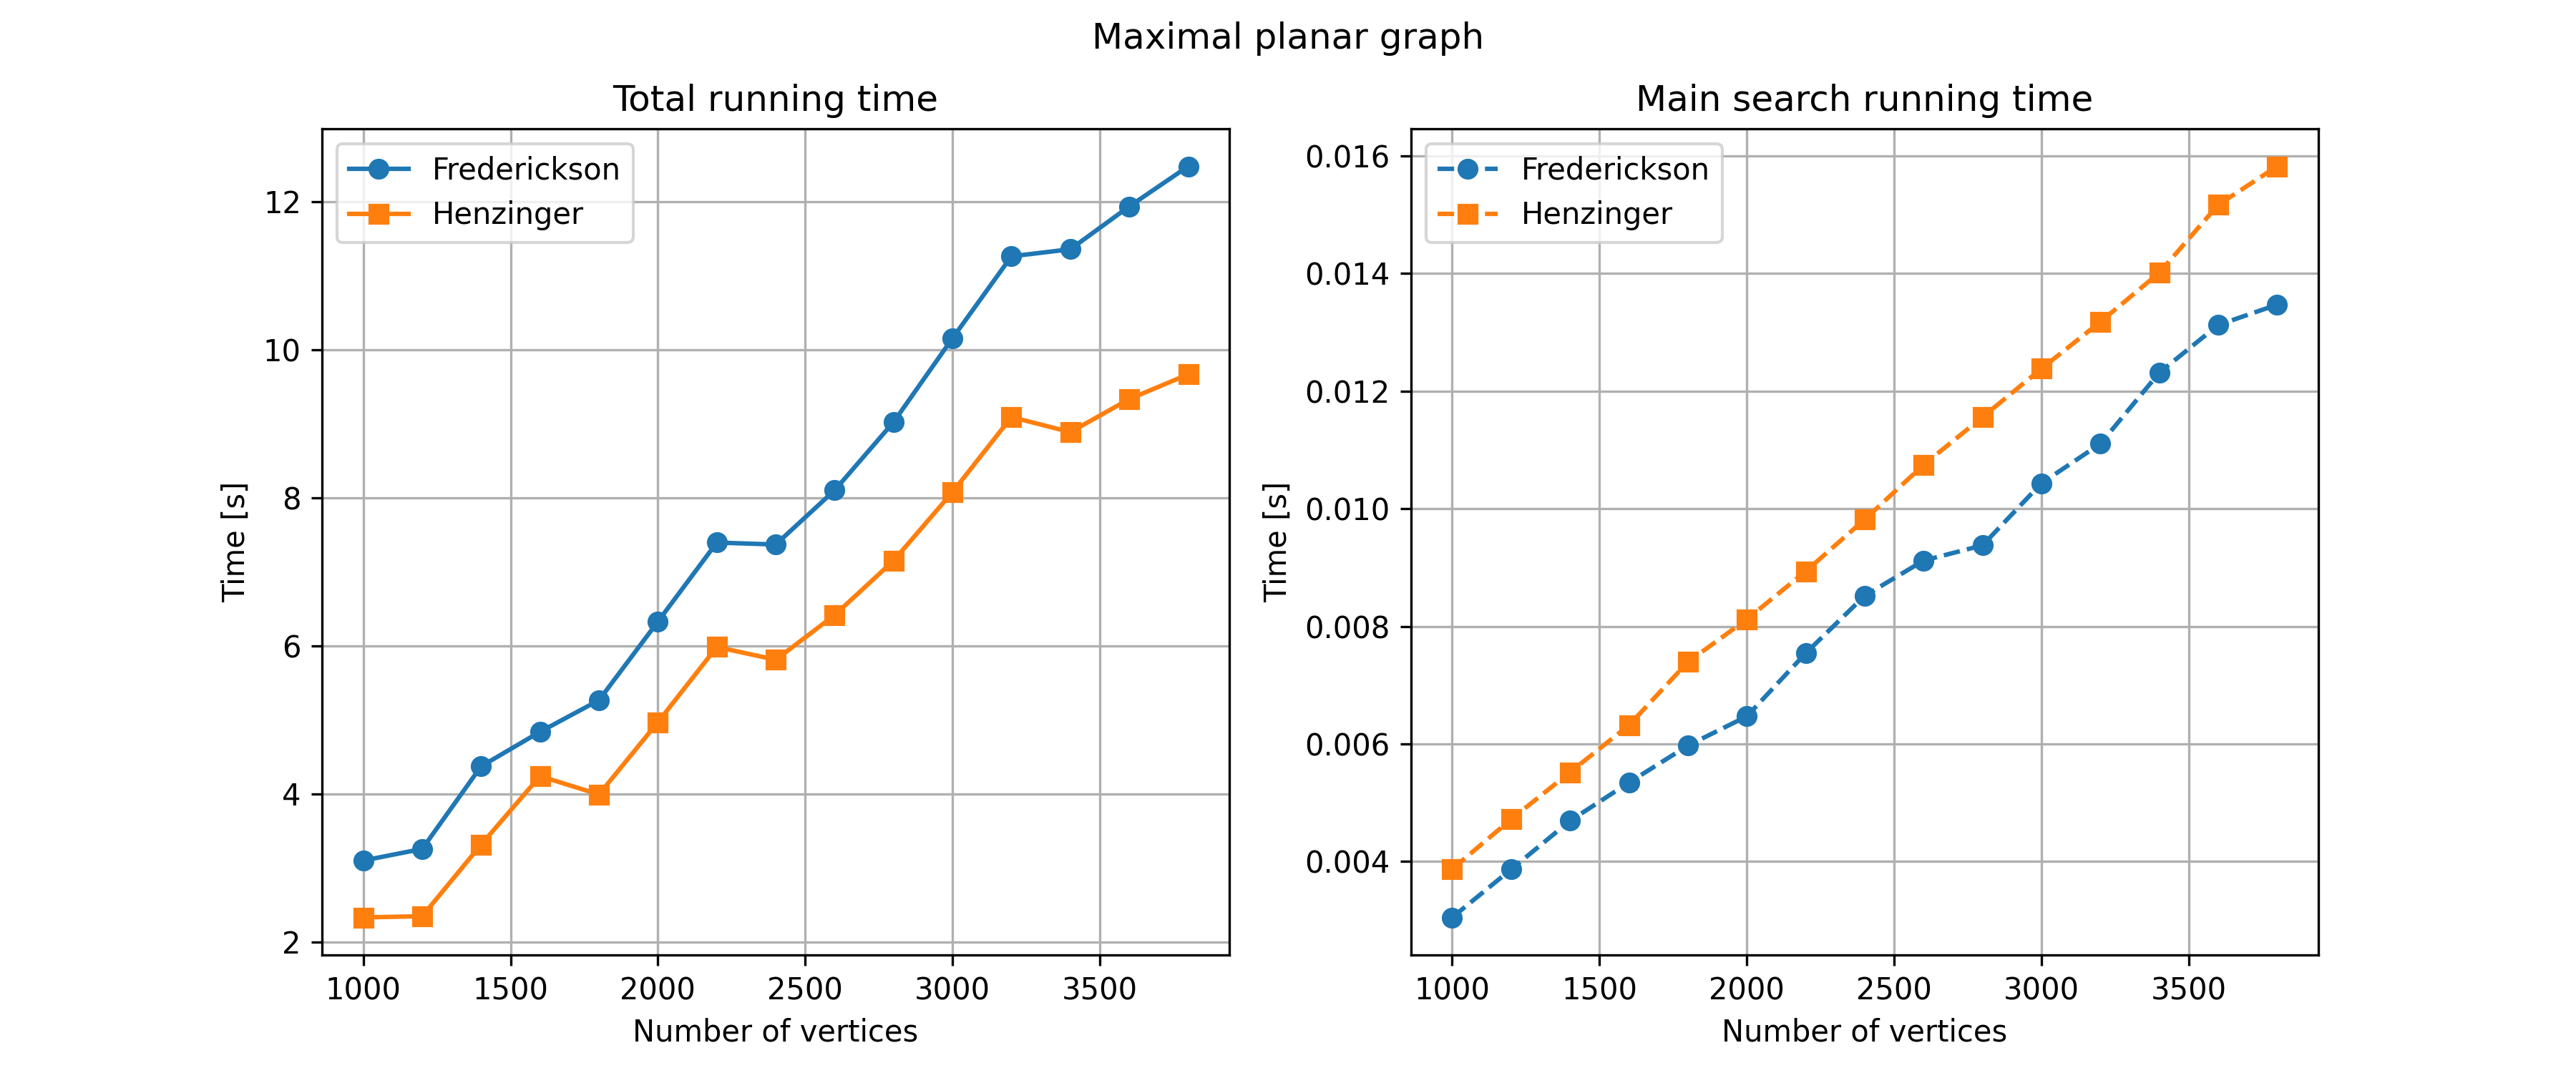
\includegraphics[width=1.4\textwidth]{charts/max.png}
    \end{adjustbox}
    \caption{}
    \label{fig:max}
\end{figure}

\begin{figure}[H]
    \centering
    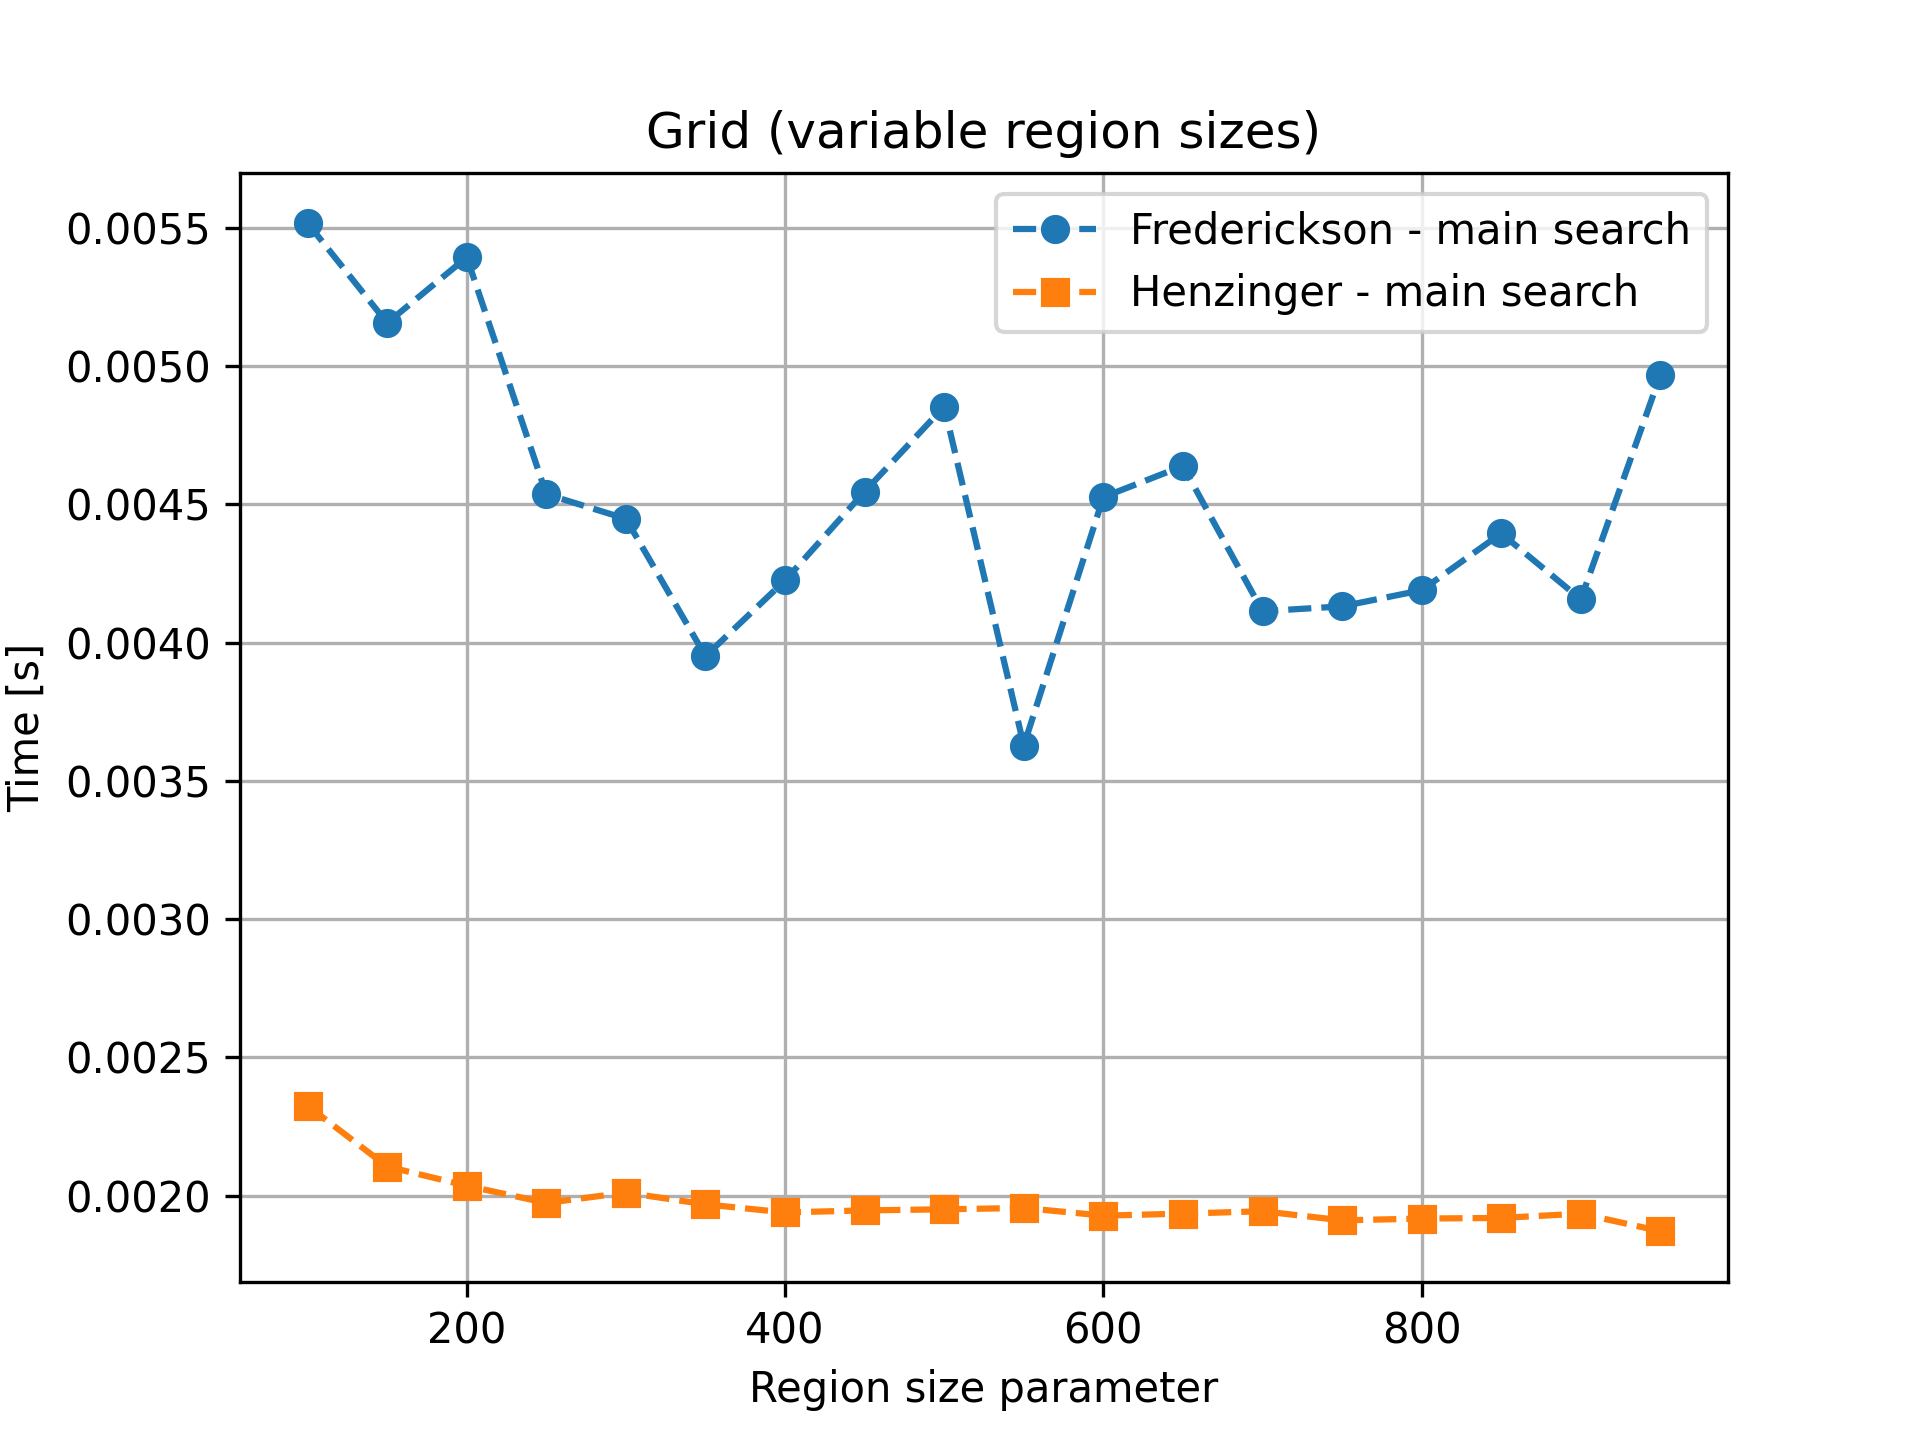
\includegraphics[width=0.9\textwidth]{charts/Pgrid.png}
    \caption{}
    \label{fig:Pgrid}
\end{figure}

\begin{figure}[H]
    \centering
    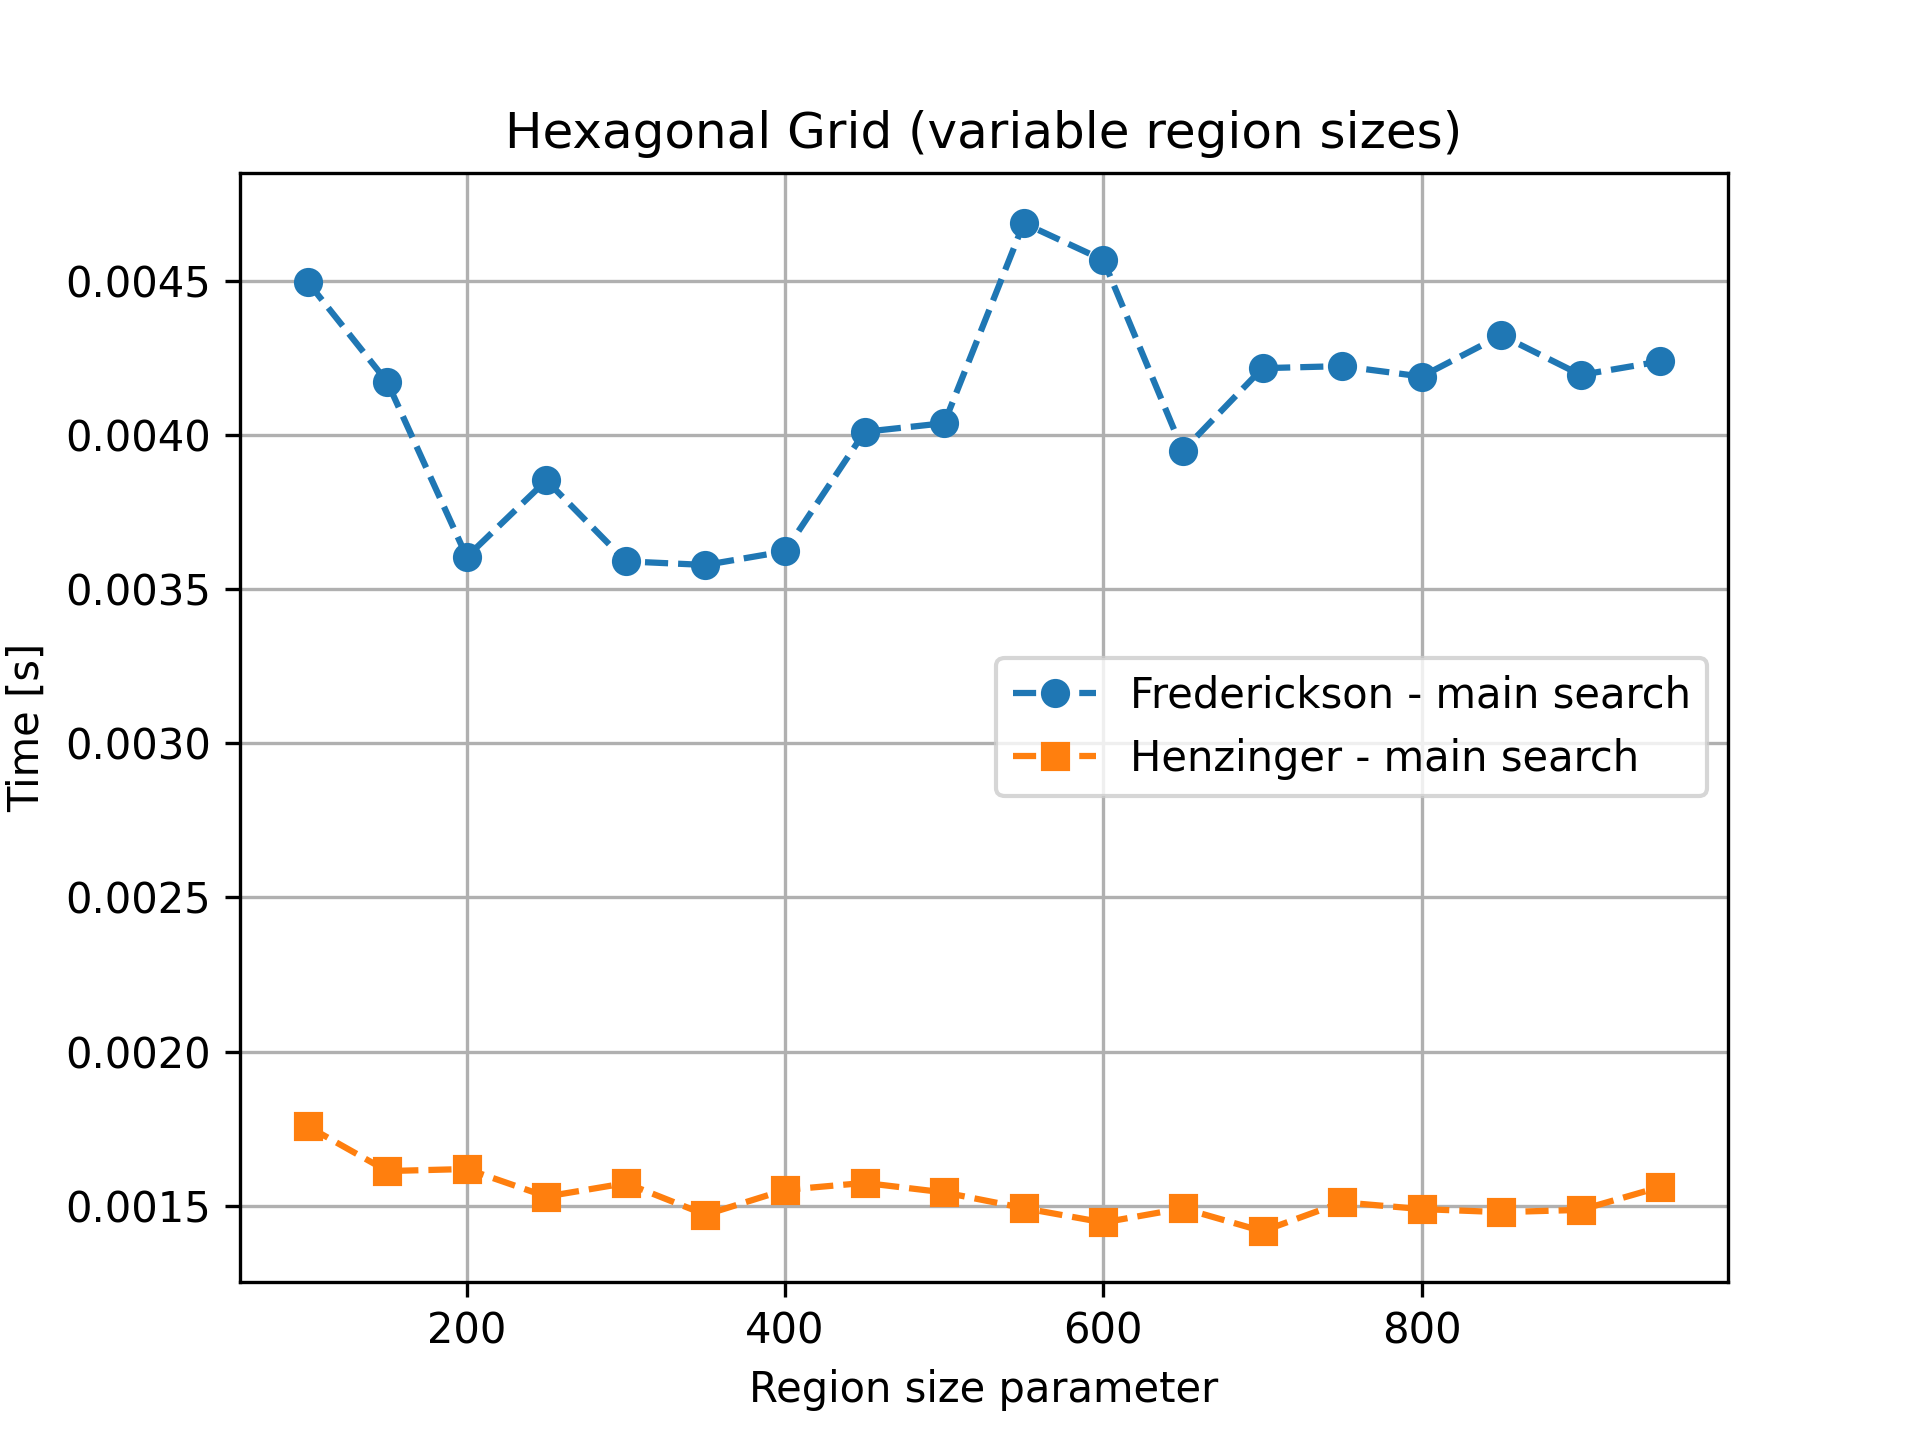
\includegraphics[width=0.9\textwidth]{charts/Phex.png}
    \caption{}
    \label{fig:Phex}
\end{figure}

\begin{figure}[H]
    \centering
    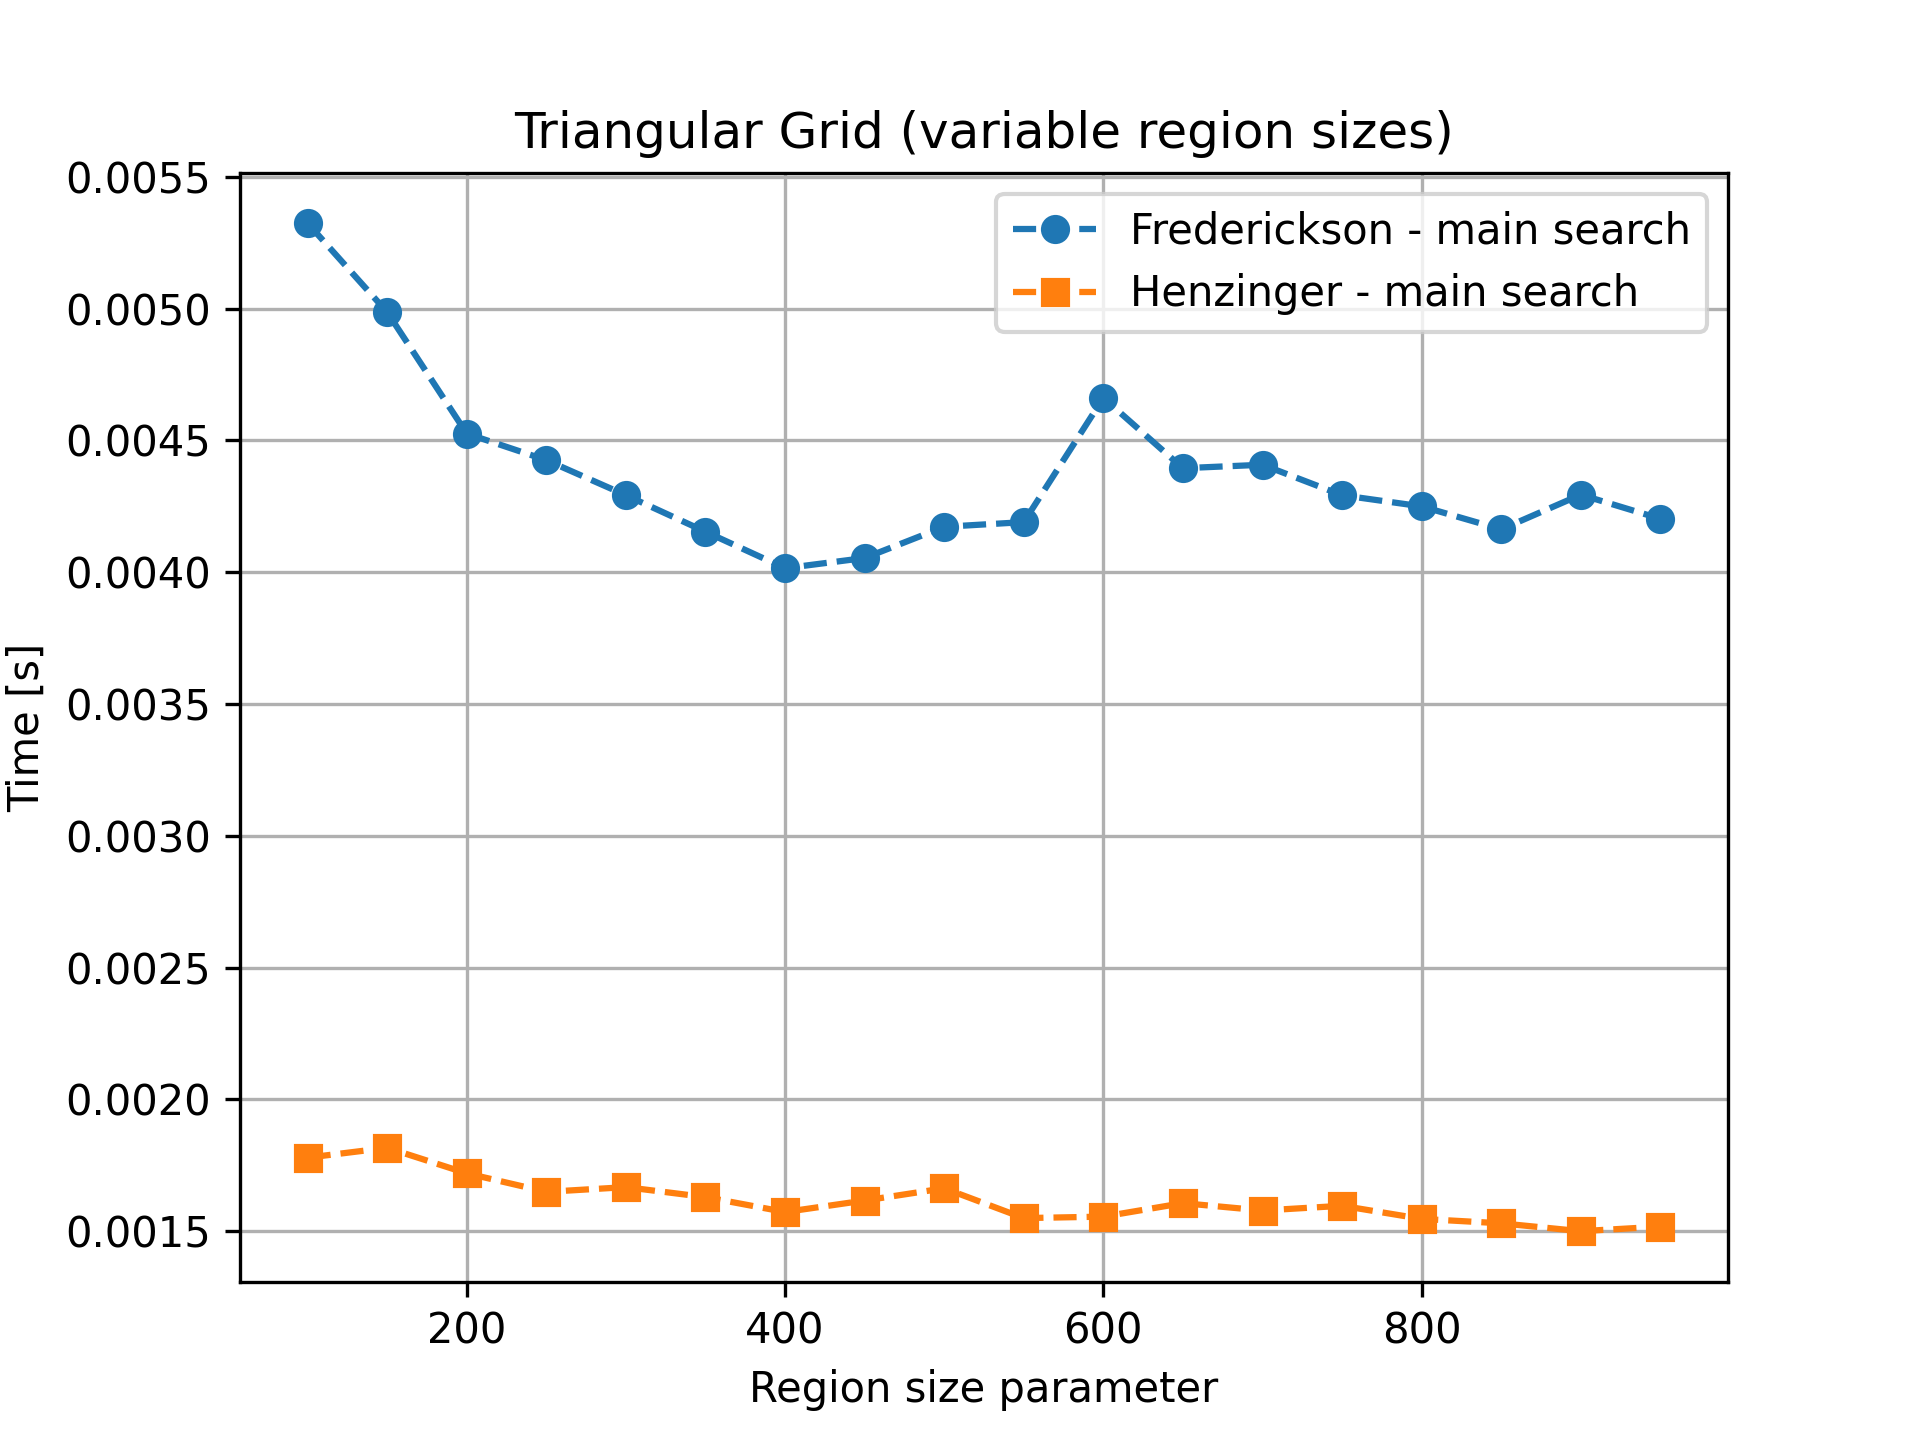
\includegraphics[width=0.9\textwidth]{charts/Ptrig.png}
    \caption{}
    \label{fig:Ptrig}
\end{figure}

\begin{figure}[H]
    \centering
    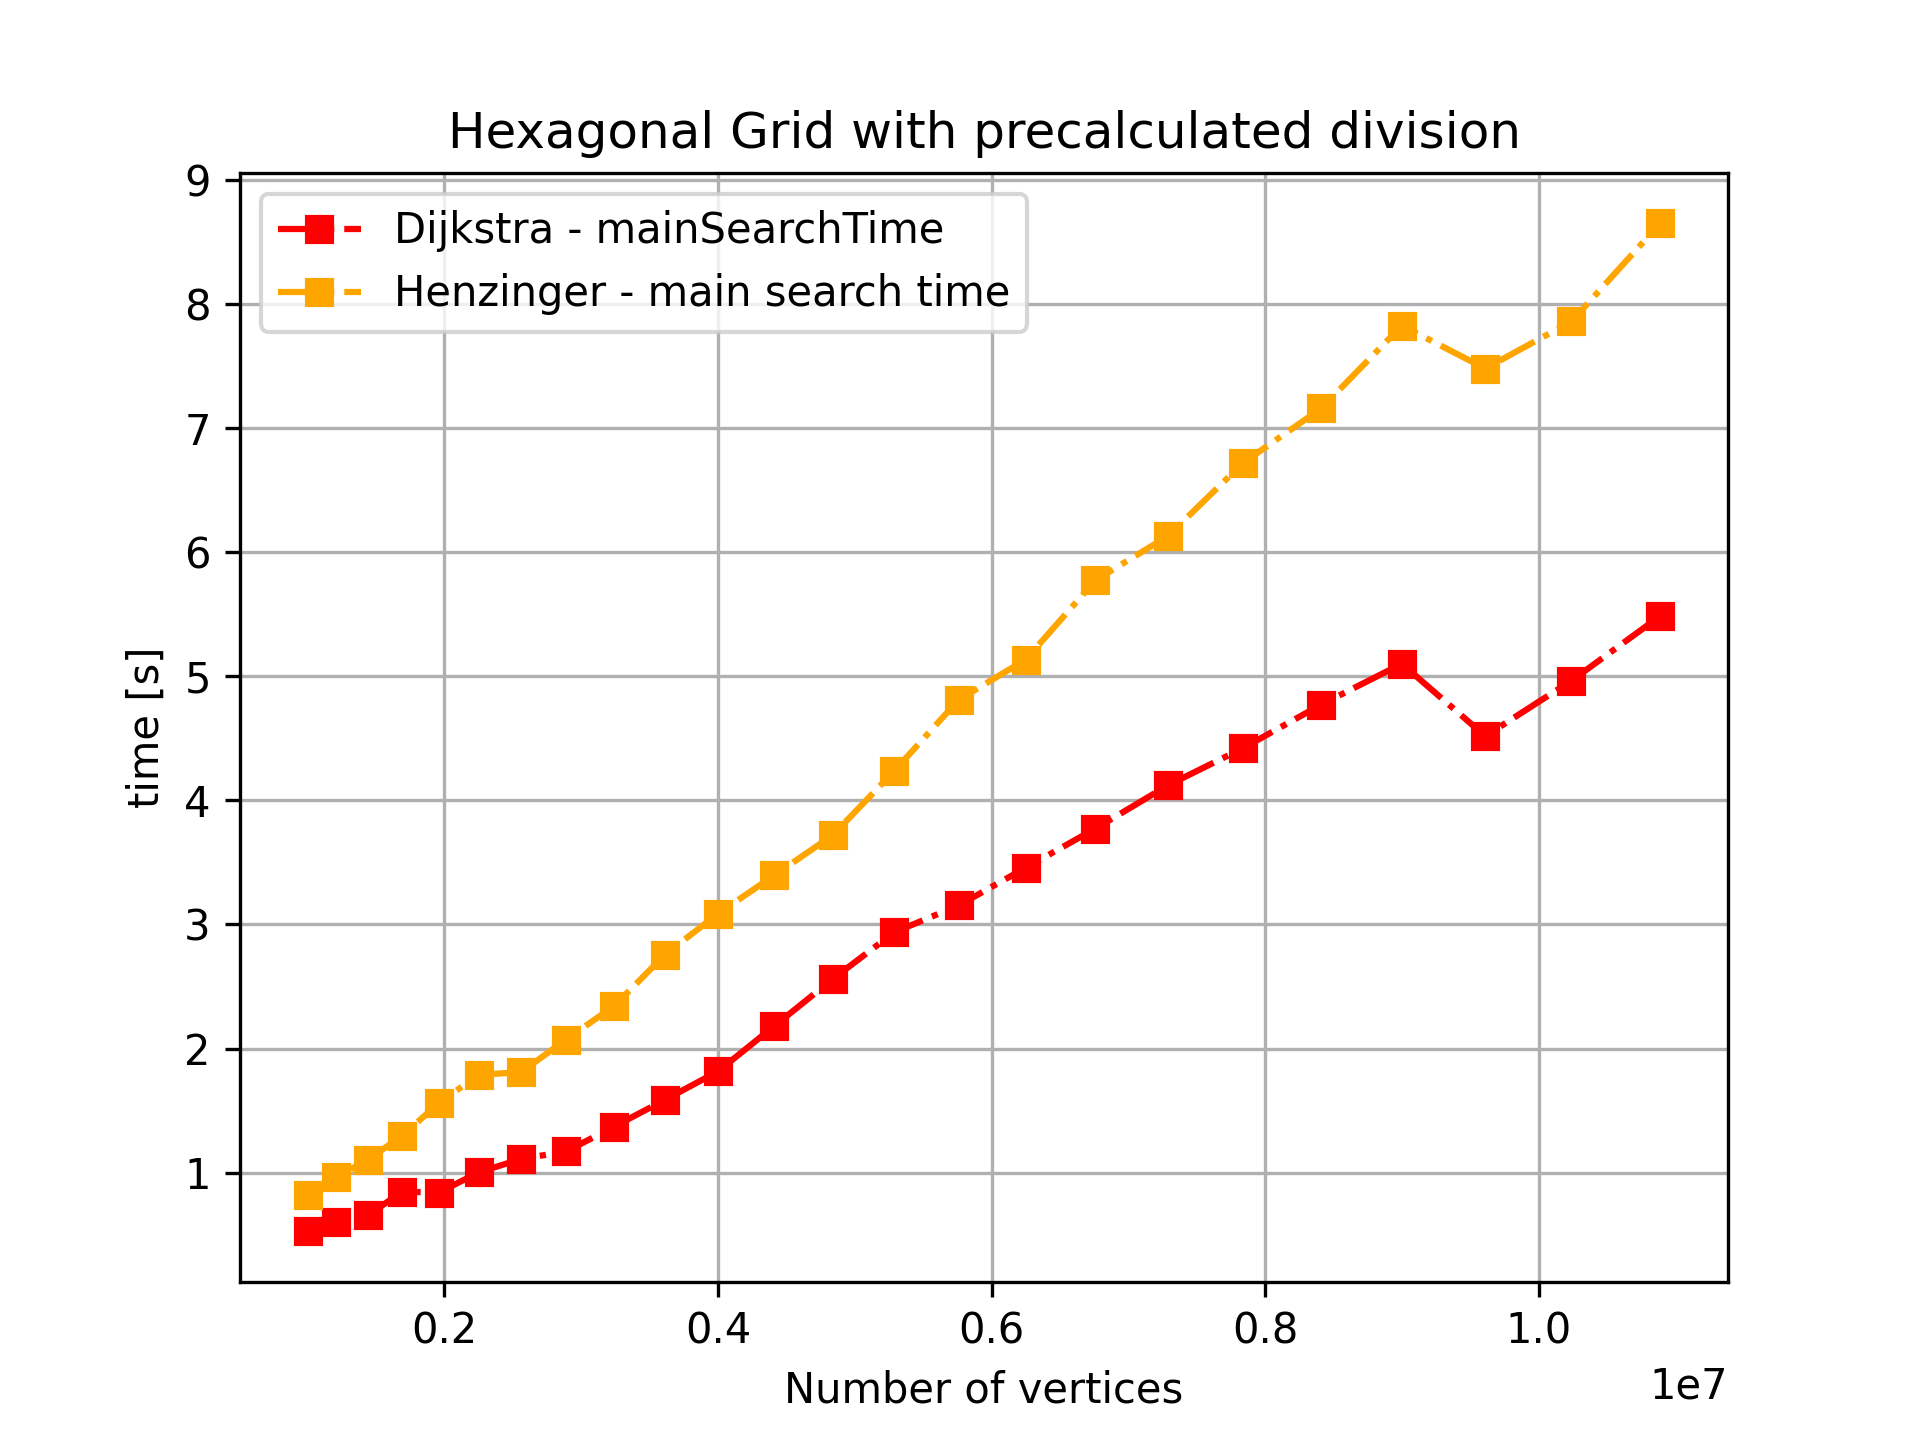
\includegraphics[width=0.9\textwidth]{charts/PrecalculatedHenzinger.png}
    \caption{}
    \label{fig:PrecalculatedHenzinger}
\end{figure}

The time measurements in the benchmarks were divided into the total running time and the running time of the main search phase only, as the main contributing factor to the total running time was generating the division. The difference between the full running time and the main search phase time was primarily due to the implementation of the separator algorithm.

From the benchmarks, we can conclude that Henzinger's algorithm is faster for denser graphs, although its running time on maximal planar graphs (see \Cref{fig:max}) is comparable to Frederickson's algorithm, with a slight advantage for Frederickson. Even though all graphs were transformed to have bounded degree, the underlying structure of the graph still impacts performance after the transformation. The main search phase of Frederickson's algorithm runs faster on very sparse graphs such as line graphs(see \Cref{fig:line}), but its total running time is significantly worse in all cases compared to Henzinger's algorithm. This is likely due to the extra level of division, smaller parameter sizes, and the dominating effect of the separator algorithm implementation. Benchmarks on subgraphs of the real New York City map (see \Cref{fig:city}) further confirm that the structure of the graph has a significant impact on the running time of the algorithms, resulting in considerable variation in the measured sample times.